\documentclass[useAMS]{mn2e}
\usepackage{graphicx}

\title[]{BEST-2 Specifications}

\begin{document}

\pagerange{\pageref{firstpage}--\pageref{lastpage}} \pubyear{2011}

\maketitle


\begin{figure}
    \centering
    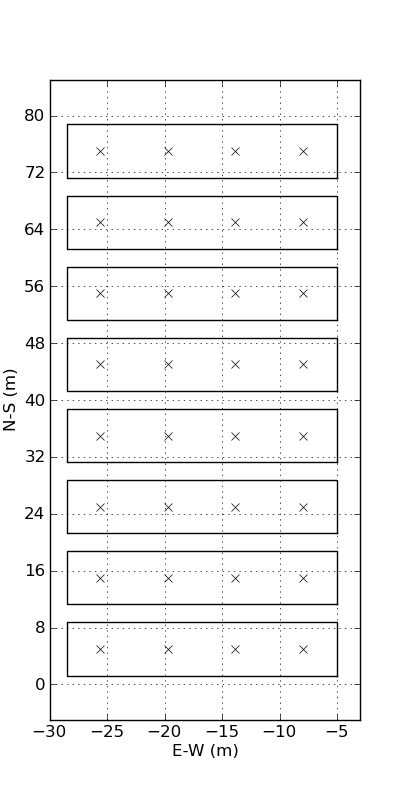
\includegraphics[scale=0.4]{layout.png}
    \caption{BEST-2 8 cylinder array layout}
\end{figure}

\begin{figure}
    \centering
    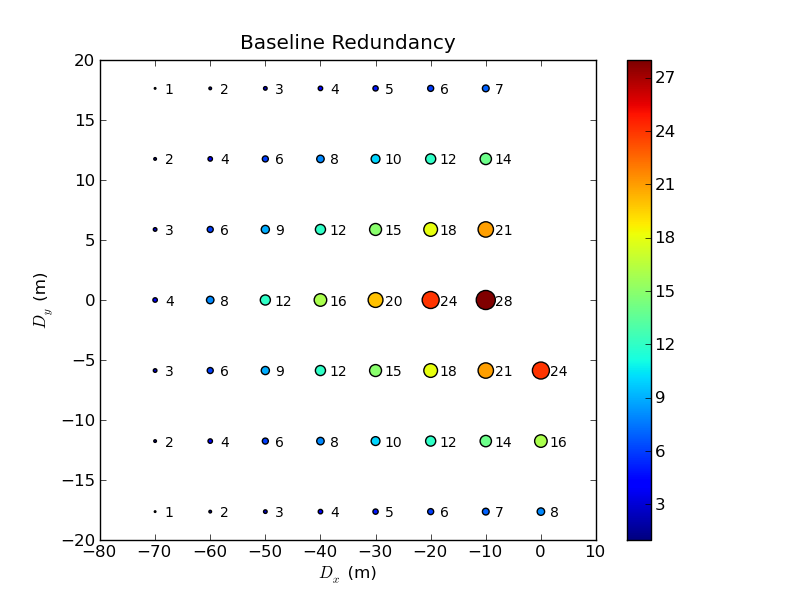
\includegraphics[scale=0.4]{redbl.png}
    \caption{Color and size represent the redundancy of a baseline}
\end{figure}

%__________________________________________________ One column table
   \begin{table}
         \label{BEST2_spec}
     $$ 
         \begin{array}{p{0.5\linewidth}rl}
            \hline
            \noalign{\smallskip}
            %-------------------------------------------
		Cylinder Properties & &\\
		\hline
		Number of RX per cylinder &          4 &            \\

		Cylinder diameter &        7.5 &          m \\

		Cylinder lenght &       23.5 &          m \\

		Element diameter &        7.5 &          m \\

		Element lenght &       5.88 &          m \\

		Element collecting area &       44.1 &        m^2 \\

		Aperture efficiency &       0.71 &            \\

		Element effective area &     31.311 &        m^2 \\

		           &            &            \\
		\hline
		BEST-2 &            &            \\
		\hline
		Number of cylinder &          8 &            \\
		Total number of RX &         32 &            \\
		Total collective area &     1411.2 &        m^2 \\
		Total effective area &    1001.95 &        m^2 \\
		Sensitivity / Ant. gain &       0.36 &       K/Jy \\
		Aeff/Tsys &      11.65 &      m^2/K \\
		Antenna temperature &         35 &          K \\

		Receiver temperature &         51 &          K \\

	    System temperature  &         86 &          K \\

		           &            &            \\
		\hline
		Longest baseline &            &            \\
		\hline
	      	E/W &      17.04 &         m \\
	       	N/S &      70.00 &         m \\
		           &            &            \\
		\hline
		Bandpass        &           &       \\
        \hline
		Central frequency &        408 &        MHz \\

		Analog BW &         16 &        MHz \\

		Digital BW &         20 &        MHz \\

        Channels &          1024 &          \\

        Channel Resolution &    19.53 &     kHz \\

		           &            &            \\
		\hline
		Pointing Limits &            &            \\
		\hline

		declination &    (0,+90) &        deg \\
		
        right ascension &    \textrm{local meridian} &  \\

		           &            &            \\
		\hline
		Primary Beam &          &           \\
        \hline
		Primary beam size &      37.62 &      deg^2 \\

		declination &        5.7 &        deg \\

		right ascension &        6.6 &        deg \\

		           &            &            \\
		\hline
		Synthesized Beam    &       &       \\
        \hline
		Synthesized beam size &        0.9 &      deg^2 \\

		declination &       0.52 &     deg \\

		right ascension &        1.73 &     deg \\
		           &            &            \\
		\hline
		Correlator    &       &       \\
        \hline
        Baselines       &       496 &   \\
        Integration time (min)  &  6.5  &   ms  \\ 

            
            %-------------------------------------------
         \end{array}
     $$ 
   \end{table}
\end{document}
